\documentclass[12pt]{article}

\usepackage{graphicx}
\usepackage{paralist}
\usepackage{listings}
\usepackage{booktabs}
\usepackage{hyperref}
\usepackage{amsmath}
\graphicspath{ {./img/} }

\oddsidemargin 0mm
\evensidemargin 0mm
\textwidth 160mm
\textheight 200mm

\pagestyle {plain}
\pagenumbering{arabic}

\newcounter{stepnum}

\title{Greedy Algorithm Drasil Case Study}
\author{Don Chen}
\date{\today}

\begin {document}

\tableofcontents

\section{Reference Material}
This section records information for easy reference.

\section{Problem Description}
In the real world, we are facing a lot of optimization problem. For example:
A saleman would like to travel all the cities in the Great Toronto Area to promote companies products.
This person does not want to visit the city two times. What is the shortest possible route that visits 
each city exactly once? This problem can also apply to logistics and telecommunication.
Find the most optimized solution usually will bring the cost down.

\section{General System Description}
% This section provides general information about the system including identifying the interfaces between the system 
% and its environment (system context), describing the user characteristics and listing the system constraints.

\section{Specific System Description}
% This section first presents the problem description, which gives a high-level view of the problem to be solved. 
% This is followed by the solution characteristics specification, which presents the assumptions, theories, theoretical 
% models, general definitions, data definitions, and finally the instance models that model the weighted graph.

\subsection{General Definition}
\begin{itemize}
    \item v vertex: a basic unit(such a city) disperse in a graph.
    \item V vertices: a set of vertices.
    \item e edge: a connction bewteen two vertices.
    \item E edges: a set of edges.
    \item G graph: A graph G is an ordered triple (V, E, f) consisting of a nonempty set V of vertices, 
    a set E of edges, and an incidence function f that associates with each edge and two vertices.
    \item f relation function bewteen e and v: If e is an edge and u and v are vertices, 
    u, v $\in$  V, such that f(e) = u$\sim$v, then e is said to join u and v; u and v are endpoints of edge e.     
    \item G = (V, E, f, w) is a weighted graph: A weighted graph is a graph with each edge e of G let there be associated a real number w(e).
    \item w: E$\rightarrow\Re$ Weight: With each edge e of G let there be associated a real number w(e).
    \item ve: either a vertex or an edge
    \item VE: a set of ve
\end{itemize}

\subsection{Graph in Drawing}
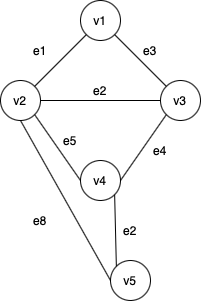
\includegraphics[scale=0.5]{graph.png}

\subsection{Example of a Weighted Graph}
\begin{itemize}
    \item G = (V(G), E(G), f, w)
    \item V = \{$v_1$, $v_2$, $v_3$, $v_4$, $v_5$\}
    \item E = \{$e_1$, $e_2$, $e_3$, $e_4$, $e_5$, $e_6$, $e_7$, $e_8$\}
    \item f($e_1$) = $v_1\sim v_2$, f($e_2$) = $v_2\sim v_3$, f(e3) = $v_1\sim v_3$, f(e4) = $v_3\sim v_4$, 
    \item f(e5) = $v_2\sim v_4$, f($e_6$) = $v_4\sim v_5$, f($e_7$) = $v_2\sim v_5$, f($e_8$) = $v_2\sim v_5$
    \item w($e_1$) = $n_1$, w($e_2$) = $n_2$, w($e_3$) = $n_3$, w($e_4$) = $n_4$,
    \item w($e_5$) = $n_5$, w($e_6$) = $n_6$, w($e_7$) = $n_7$, w($e_8$) = $n_8$ where $n\in\Re$
\end{itemize}

\subsection{Goal Statements}
Give a weighted graph, the goal statements are:
\begin{itemize}
    \item Find the shorest path where all vertices appear only once in a path.
    \item Find the total weight of the shorest path.
\end{itemize}

\subsection{Assumptions}
\begin{itemize}
    \item V and E are finite sets.
    \item It is undirected graphs, means f(e) = u$\sim$v = v$\sim$u.
    \item It is a connected graph.
    \item There is no loop in the graph.
\end{itemize}

\subsection{Theoretical Model}
Minimize(\{p:Path $|$ p$\in$SP: TotalWeight(p)\})

\begin{itemize}
    \item SetVE $\equiv V || E$
    \item AllCombinaiton $\equiv \cup(x: ve | x\in SetVE: \{Combine(x)\})$
    \item Combine(a,b) $\equiv$ [a$||$b]
    \item SW := 
    $$\{x, i: VE, N| x \in AllCombinaiton \wedge 1 \le i \le length(x) \wedge f(x[i]) = x[i-1]\sim x[i] : x\}$$
    \item length(x) $\equiv$ +(y:VE $|$y$\in$x: 1)
    \item SP :=
    $$\{w:Walk | w\in SW: \forall (x: Walk | x \in SW: IsDistinctV(x) \wedge IsDistinctE(x) \wedge IsVisitAllV(x))\}$$
    \item IsDistinctV(x) $\equiv$ (+(v:vertice $|$ v$\in$x: 1) == +(v:vertice $|$ v$\in$SetofVertice(x): 1))
    \item IsDistinctE(x) $\equiv$ (+(e:edge $|$ e$\in$x: 1) == +(e:edge $|$ e$\in$SetofEdge(x): 1))
    \item IsVisitAllV(x) $\equiv$ (+(v:vertice $|$ v$\in$V: 1) == +(v:vertice $|$ v$\in$SetofVertice(x): 1))
    \item SetofEdge(x) $\equiv \cup$(e:edge $|$ e$\in$E: \{e\})
    \item SetofVertice(x)$\equiv \cup$(v:vertice $|$ v$\in$x: \{v\})
    \item TotalWeight(p) $\equiv$ +(e:edge $|$ e$\in$p: w(e))
    \item Minimize(TWs) $\equiv (w \in TWs) \wedge \forall (x :R | x \in TWs : w \le x)$
\end{itemize}

\subsection{Supporting Data Definitions}
\begin{itemize}
    \item A graph G is connected if for every u, v $\in$ V there exists a path connect u and v in G. 
    Otherwise G is called disconnected.
    \item Finite Graph: A graph is finite if both its set of vertices and set of edges are finite.
    \item Endpoint: if f(e) = u$\sim$v, edge e has endpints of u and v. u and v $\in$  V(G).
    \item Loop: An edge with identical ends. f(e) = vu and v = u. u and v $\in$  V(G).
    \item Connected Graph: if for every u, v $\in$ V there exists f(e) = u$\sim$v. Otherwise G is called disconnected.
    \item Walk: A walk is a well formed sequence W = $<v_0$, $e_1$, $v_1$, $...$, $e_k$, $v_k>$, 
    whose terms are alternatively vertices and edges such that for 1$\le$i$\le$k, 
    the edge $e_i$ has endpoints $v_{i-1}$ and $v_i$. f($e_i$) = $v_{i-1}v_i$. k is the length of W.
    \item Trail: If the edges $e_1$, $e_2$, $...$, $e_k$ of a walk are distinct.
    \item Path: a path is a walk if both of its edges $e_1$, $e_2$, $...$, $e_k$ 
    and its vertices $v_0$, $v_1$, $...$ , $v_k$ are distinct.
    % \item Closed: A u,v-walk has first vertex u and last vertex v. 
    % When the first and last vertex of a walk, trail or path are the same, we say that they are closed. 
    % \item Cycle:
\end{itemize}

\subsection{Instance Models}
\begin{itemize}
    \item Input: G = (V, E, f, w)
    \item Output: a sequence
\end{itemize}

\section{Likely Changes}
\begin{itemize}
    \item There could be new algorithms to solve graph problems
\end{itemize}

\section{Unlikely Changes}
\begin{itemize}
    \item The final output is the most optimal result, it is unlikely change.
\end{itemize}

\section{Algorithm}
\subsection{Kruskal’s Algorithm}
Given G = (V, E, f, w) 
\begin{itemize}
    \item initialize F = (V, $\oslash$)
    \item for edges e in increasing order of length w
    \item if edges e are do not form a cycle with F
    \item $\dots\dots$\{add e to F\}
    \item return F
\end{itemize}

\subsection{Pseudo Code in Drawing}
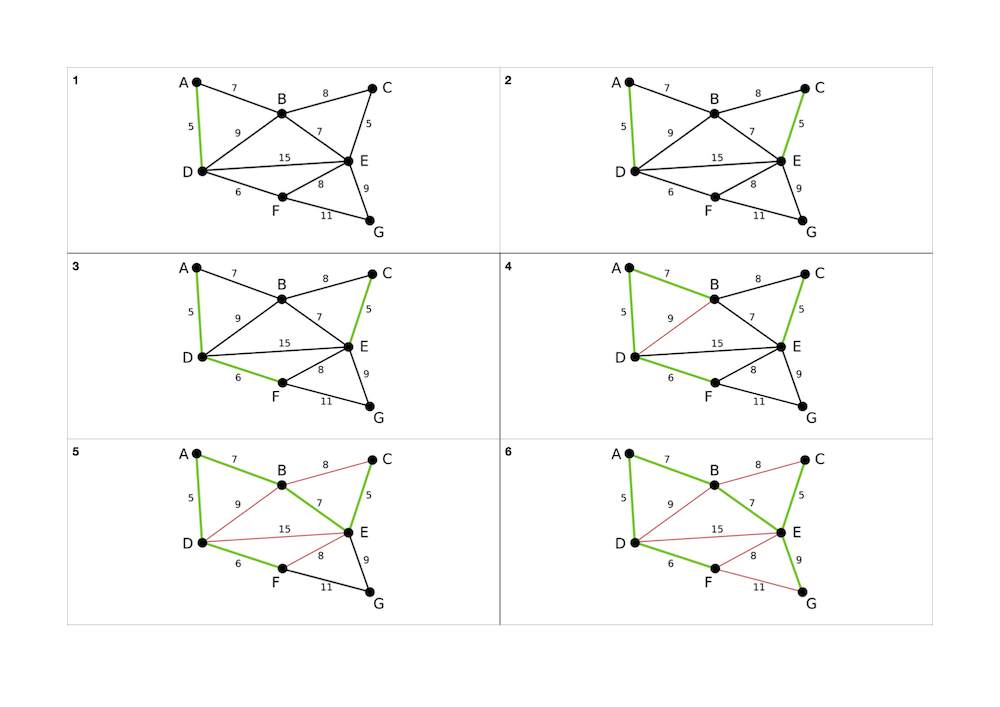
\includegraphics[scale=0.5]{kruskalalgorithm.png}

\subsection{Nearest Neighbor Alorithm(usually can't find an optimized solution)}

\section{Question}
\begin{itemize}
    \item well formed sequence such as
\end{itemize}

\section{Reference}
\begin{itemize}
    \item Graph Theory With Applications by J.A. Bondy and U. S. R. Murty
    \item \href{http://math.mit.edu/~goemans/18433S15/TSP-CookCPS.pdf}{Nearest Neighbor Alorithm} 
    \item \href{https://www.ams.org/journals/proc/1956-007-01/S0002-9939-1956-0078686-7/home.html}{Kruskal  Alorithm in TSP} 
\end{itemize}

\end {document}